\documentclass[a4paper]{article}
\usepackage[spanish,es-tabla]{babel}	% trabajar en español
\spanishsignitems	
%\usepackage{simplemargins}

%\usepackage[square]{natbib}
\usepackage{amsmath}
\usepackage{amsfonts}
\usepackage{amssymb}
\usepackage{bbold}
\usepackage{graphicx}
\usepackage{blindtext}
\usepackage{hyperref}
\usepackage{amsthm}
\newtheorem{theorem}{Teorema}
\newtheorem{lemma}{Lema}
\usepackage{algorithm}
%\usepackage{algorithmic}
\usepackage{algpseudocode}
%\usepackage{algorithm2e}
\usepackage{booktabs}

\setcounter{MaxMatrixCols}{20}

\begin{document}
\pagenumbering{arabic}

\Large
 \begin{center}
\textbf{Método de Elementos Finitos}\\


\hspace{10pt}

% Author names and affiliations
\large
%Lic. Julio A. Medina$^1$ \\
Julio A. Medina\\
\hspace{10pt}
\small  
Universidad de San Carlos\\
Escuela de Ciencias Físicas y Matemáticas\\
Maestría en Física\\
\href{mailto:julioantonio.medina@gmail.com}{julioantonio.medina@gmail.com}\\

\end{center}

\hspace{10pt}

\normalsize
\section{Introducción al Método de Elementos Finitos}
Este método para aproximar las soluciones de ecuaciones diferenciales parciales fue originalmente desarrollado para su uso en problemas de ingeniería civil pero en la actualidad su uso es ubicuo para aproximar soluciones en todas las áreas de la matemática aplicada y en muchas aplicaciones de la física. Su uso es intensivo en el modelado de sistemas complejos para el diseño aerodinámico de piezas y dispositivos de exploración espacial así como también en aplicaciones avanzadas de la ingeniería como las competiciones automovilísticas en el caso de la Formula 1. \\ 

Una de las ventajas del método de elementos finitos sobre el método de diferencias finitas es la relativa facilidad con la que el método de elementos finitos maneja las condiciones de frontera. Muchos problemas físicos(pragmáticos) tienen condiciones de frontera que involucran derivadas y contornos de formas irregulares, sin simetrías aparentes. Condiciones de frontera de este tipo son difíciles de manejar con los métodos de diferencias finitas ya que cada condición de frontera que involucra a alguna derivada tiene que aproximarse con un cociente de diferencias en los puntos del retículo o malla, pero el hecho que se tienen bordes irregulares hace que la definición de un retículo adecuado sea poco trivial. El método de diferencias finitas por el otro lado incluye a las condiciones de frontera como integrales en un funcional que debe minimizarse, de esta manera la construcción del procedimiento del método de elementos finitos es independiente de las condiciones particulares de frontera del problema.\\

La ecuación diferencial parcial a atacar es la siguiente
\begin{equation}\label{eq::partial_diff_equation}
\frac{\partial}{\partial x}\Bigg( p(x,y)\frac{\partial u}{\partial x} \Bigg) + \frac{\partial}{\partial y}\Bigg( q(x,y)\frac{\partial u}{\partial y} \Bigg) +r(x,y)u(x,y)=f(x,y)
\end{equation}
con $(x,y)\in \mathcal{D}$, donde $\mathcal{D}$ es una región plana con frontera $\mathcal{S}$.\\

Condiciones de frontera de la forma
\begin{equation}\label{eq::boundary1}
u(x,y)=g(x,y)
\end{equation}
se imponen en una porción $\mathcal{S}_1$ de la frontera. En el resto de la frontera, $\mathcal{S}_2$, se requiere que la solución satisfaga
\begin{equation}\label{eq:boundary2}
p(x,y)\frac{\partial u}{\partial x}(x,y)\cos\theta_1+q(x,y)\frac{\partial u}{\partial y}(x,y)\cos\theta_2+g_1(x,y)u(x,y)=g_2(x,y),
\end{equation}
donde $\theta_1$ y $\theta_2$ son los ángulos de dirección de las normales salientes en el punto $(x,y)$, ver figura \ref{fig::fig1}
\begin{figure}[h]
\begin{center}
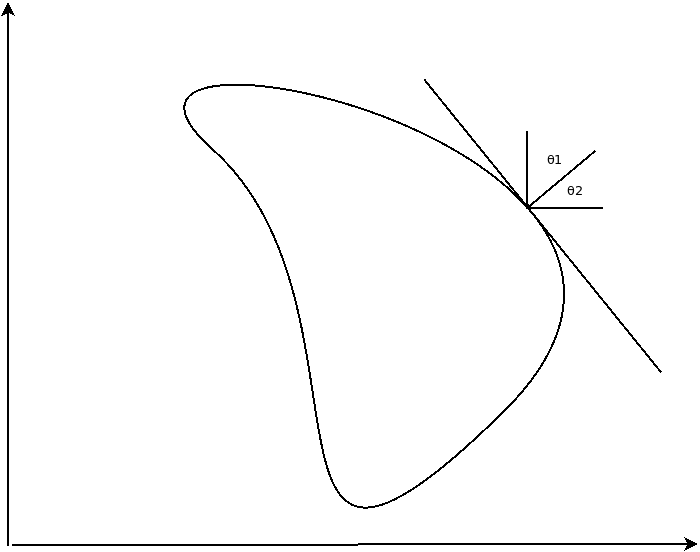
\includegraphics[scale=0.42]{./fig1.png} 
\end{center} 
\caption{Visualización ángulos $\theta_1$ y $\theta_2$}
\label{fig::fig1}
\end{figure}
Algunos problemas en física en áreas como mecánica de sólidos y elasticidad tienen ecuaciones diferenciales parciales asociadas similares a \ref{eq::partial_diff_equation}. La solución a este problemas de este tipo típicamente minimizan cierto funcional, que involucra integrales definidas, sobre una clase de funciones determinada por el problema.\\

Al suponer que $p,q,r$ y $f$ son todas continuas en $\mathcal{D}\cup\mathcal{S}$, $p$ y $q$ tiene primeras derivadas parciales continuas, y $g_1$ y $g_2$ son continuas en $\mathcal{S}_2$. Adicionalmente se supone que $p(x,y)>0, \, q(x,y)>0,\,r(x,y)\leq 0$ y $g_1(x,y)>0$. Entonces la solución de \ref{eq::partial_diff_equation} minimiza el funcional $I[w]$ únicamente, i.e. está es la única función que minimiza al funcional.
\begin{equation}\label{eq::functional}
\begin{aligned}
I[w]=\int\int_{\mathcal{D}}\Bigg\{ \frac{1}{2}\Big[p(x,y)\Big( \frac{\partial w}{\partial x} \Big)^2 + q(x,y)\Big( \frac{\partial w}{\partial y} \Big)^2 -r(x,y) w^2 \Big] +f(x,y)w\Bigg\}dx dy\\
+\int_{\mathcal{S}_2}\Bigg\{ -g_2(x,y)w+\frac{1}{2}g_1(x,y)w^2 \Bigg\}dS
\end{aligned}
\end{equation}
sobre todas las funciones dos veces diferenciables y continuas $w$ que satisfacen la ecuación \ref{eq::boundary1} en $\mathcal{S}_1$. El método de elementos finitos aproxima está solución al minimizar al funcional I \ref{eq::functional} sobre una clase mas pequeña de funciones, similar al acercamiento utilizado el método de Rayleigh-Ritz(ver Burden. \cite{Burden}).
\subsection{Definiendo los elementos finitos}
El primer paso es de definir los elementos finitos para construir la aproximación, esto consiste en dividir la región en un número finito de secciones o elementos con una forma regular, pueden ser triángulos, rectángulos, o cualquier figura regular que "tesele"  la región por completo(\textit{tiling the region}).\\

El conjunto de funciones regularmente usadas para la aproximación es un conjunto de polinomios por partes de grado fijo en $x$ y $y$, y la aproximación requiere que los polinomios sean unidos de tal manera que la función resultante sea continua con primera y segunda derivadas integrables sobre la región entera. polinomios de tipo linear en $x$ y $y$ 
\begin{equation}
\phi(x,y)=a+bx+cy
\end{equation}
se utilizan comúnmente con elementos triangulares, mientras que polinomios de tipo bilinear en $x$ y $y$
\begin{equation}
\phi(x,y)=a+bx+cy+dxy
\end{equation}
están asociados al uso de elementos rectangulares.\\

Suponiendo que la región $\mathcal{D}$ ha sido subdividida en elemento triangulares. El conjunto de triángulos se denota como $D$, y los vértices de dichos triángulos se llaman nodos. El método busca una aproximación de la forma 
\begin{equation}
\phi(x,y)=\sum_{i=1}^{m}\gamma_i \phi_i(x,y),
\end{equation}
donde $\phi_1,\phi_2,\hdots,\phi_m$ son polinomios lineales por partes linealmente independientes, y las $\gamma_1, \gamma_2,\hdots,\gamma_m$ son constantes. Algunas de estas constantes, por ejemplo $\gamma_{n+1}, \gamma_{n+2},\hdots,\gamma_m$ se utilizan para asegurar que la condición de frontera 
\begin{equation}\label{eq::phi}
\phi(x,y)=g(x,y)
\end{equation}
se satisfaga en $\mathcal{S}_1$, las constantes restantes $\gamma_1,\gamma_2,\hdots,\gamma_n$, se utilizan para minimizar el funcional $I[\sum_{i=1}^m \gamma_i \phi_i]$. Usando la forma de \ref{eq::phi} para la aproximación de $w$ en la expresión \ref{eq::functional} se obtiene
\begin{equation}\label{eq::aproximated_functional}
\begin{aligned}
I[\phi]&=I\Big[ \sum_{i=1}^{m} \gamma_i \phi_i \Big]\\
&=\int\int_{\mathcal{D}}\Bigg(\frac{1}{2}\Bigg\{ p(x,y)\Big[ \sum_{i=1}^{m}\gamma_i \frac{\partial \phi_i}{\partial x}(x,y)\Big]^2 + q(x,y)\Big[ \sum_{i=1}^{m}\gamma_i \frac{\partial \phi_i}{\partial y}(x,y)\Big]^2\\
&-r(x,y)\Big[ \sum_{i=1}^{m}\gamma_i \phi_i(x,y)\Big]^2\Bigg\}+f(x,y)\sum_{i=1}^m \gamma_i \phi_i(x,y)\Bigg)dy\, dx\\
&^+\int_{\mathcal{S}_2}\Bigg\{ -g_2(x,y)\sum_{i=1}^m \gamma_i \phi_i(x,y)+\frac{1}{2}g_1(x,y)\Big[\sum_{i=1}^m \gamma_i \phi_i(x,y)\Big]^2\Bigg\}dS
\end{aligned}
\end{equation}
Como se menciono anteriormente se utiliza $\gamma_i, \gamma_2,\hdots, \gamma_n$ para minimizar el funcional, con esto al considerar a $I$ como una función de $\gamma_i, \gamma_2,\hdots, \gamma_n$, i.e. $I[\gamma_i, \gamma_2,\hdots, \gamma_n]$. Para que obtener un mínimo se tiene que cumplir
\begin{equation}\label{eq::minimun_condition}
\frac{d I}{d \gamma_j}=0,\,\, \forall\, j=1,2,\hdots,n.
\end{equation}

Diferenciando \ref{eq::aproximated_functional} con respecto $\gamma_i$ se obtiene
\begin{equation}
\begin{aligned}
\frac{\partial I}{\partial \gamma_i}=&\int \int_{\mathcal{D}}\Bigg\{p(x,y)\sum_{i=1}^m \gamma_i\frac{\partial \phi_i}{\partial x}(x,y)\frac{\partial \phi_j}{\partial x}(x,y)\\
& + q(x,y)\sum_{i=1}^{m}\gamma_i\frac{\partial \phi_i}{\partial y}(x,y)\frac{\partial \phi_j}{\partial y}(x,y)\\
& - r(x,y)\sum_{i=1}^{m}\gamma_i \phi_i(x,y)\phi_j(x,y)+f(x,y)\phi_j(x,y)\Bigg\}dx\,dy\\
& + \int_{\mathcal{S}_2}\Bigg\{-g_2(x,y)\phi_j(x,y)+g_1(x,y)\sum_{i=1}^m \gamma_i \phi_i(x,y)\phi_j(x,y)\Bigg\}dS,
\end{aligned}
\end{equation}
con esto la condición para minimizar el funcional se convierte en 
\begin{equation}
\begin{aligned}
0&=\sum_{i=1}^m \Bigg[\int \int_{\mathcal{D}}\Bigg\{ p(x,y) \gamma_i\frac{\partial \phi_i}{\partial x}(x,y)\frac{\partial \phi_j}{\partial x}(x,y)+ q(x,y) \gamma_i\frac{\partial \phi_i}{\partial y}(x,y)\frac{\partial \phi_j}{\partial y}(x,y)\\
&-r(x,y)\phi_i(x,y)\phi_j(x,y)\Bigg\}dx\,dy\\
&+ \int_{\mathcal{S}_2}g_1(x,y)\phi_i(x,y)\phi_j(x,y)dS\Bigg]\gamma_i\\
&+ \int\int_{\mathcal{D}} f(x,y)\phi_j(x,y)dx\,dy-\int_{\mathcal{S}_2} g_2(x,y)\phi_j(x,y)dS.
\end{aligned}
\end{equation}
para cada $i=1,2,\hdots,n$. Este conjunto de ecuaciones puede expresarse con una ecuación matricial
\begin{equation}
\mathbf{A}\vec{c}=\vec{b},
\end{equation}
donde $\vec{c}=(\gamma_1,\hdots,\gamma_n)^t$. Con $\mathbf{A}=(\alpha_{ij})$ y $\vec{b}=(\beta_1,\hdots,\beta_n)^t$ son definidos a continuación
\begin{equation}\label{eq::alpha_ij}
\begin{aligned}
\alpha_{ij}=\int\int_{\mathcal{D}}\Bigg[ p(x,y)\frac{\partial \phi_i}{\partial x}(x,y)\frac{\partial \phi_j}{\partial x}(x,y)+ q(x,y)\frac{\partial \phi_i}{\partial y}(x,y)\frac{\partial \phi_j}{\partial y}(x,y)\\
-r(x,y)\phi_i(x,y)\phi_j(x,y)\Bigg] dx\,dy+\int_{\mathcal{S}_2} g_1(x,y)\phi_i(x,y)\phi_j(x,y)dS,
\end{aligned}
\end{equation}
para cada $i=1,2,\hdots,n$ y $j=1,2,\hdots,m$, y
\begin{equation}\label{eq::beta_i}
\beta_i=-\int\int_{\mathcal{D}}f(x,y)\phi_i(x,y) dx\,dy+\int_{\mathcal{S}} g_2(x,y)\phi_i(x,y)dS-\sum_{k=n+1}^m\alpha_{ik}\gamma_k.
\end{equation}
para cada $i=1,\hdots,n$.\\

La elección del conjunto de funciones base es de bastante importancia ya que la elección apropiada puede frecuentemente hacer que la matriz $\mathbf{A}$ sea positiva definida y tenga la forma de una matriz banda(\textit{banded matrix}). Para el problema de segundo orden \ref{eq::partial_diff_equation}, se asume que $\mathcal{D}$ es poligonal, de tal manera que $\mathcal{D}=D$, y que $\mathcal{S}$ es un conjunto de lineas rectas contiguas.

\subsection{Triangulando la región}
Para empezar el procedimiento delineado anteriormente es crucial el paso de subdividir la región $D$ en un conjunto de triángulos  $T_1,T_2,\hdots,T_M$ donde el triángulo $i$(i-esimo) tiene tres vértices o nodos que se denotan 
\begin{equation}\label{eq::triangle_vertex}
V_j^{(i)}=\big( x_j^{(i)},y_j^{(i)} \big),\,\,\, \text{para }\, j=1,2,3.
\end{equation}
Para simplificar la notación se escribe $V^{(i)}_j=\big(x_j^{(i)},y_j^{(i)})$ cuando se trabaja con el triángulo fijo $T_i$. En cada vértice $V_j$ hay un polinomio lineal asociado
\begin{equation}
N_j^{(i)}(x,y)\equiv N_j(x,y)=a_j+b_jx+c_jy,\,\,\,\text{donde }\, N_j^{(i)}(x_k,y_k)=
\begin{cases}
1, \,\,j=k\\
0, \,\,j\neq k
\end{cases}
\end{equation}
Este esquema produce un sistema linear de la forma
\begin{equation}\label{eq::vertex_equation}
\begin{bmatrix}
1 & x_1 & y_1\\
1 & x_2 & y_2\\
1 & x_3 & y_3^
\end{bmatrix}
\begin{bmatrix}
a_j\\
b_j\\
c_j
\end{bmatrix}=
\begin{bmatrix}
0\\
1\\
0
\end{bmatrix}.
\end{equation}
En \ref{eq::vertex_equation} $j=2$ por lo que el elemento 1 ocurre en la fila 2, en general el elemento 1 ocurre en la fila $j$.\\

Sí se tienen un etiquetado de los nodos $E_1,\hdots,E_n$ que están en $D\cap \mathcal{S}$. Con cada nodo $E_k$ se asocia una función $\phi_k$ que es lineal en cada triángulo , tiene valor 1 en $E_k$, y es $0$ en los otros nodos(por construcción). Esta elección particular hace a $\phi_k$ idéntica a $N_j^{i}$ en el triángulo $T_i$ cuando el nodo $E_k$ es el vértice denotado por $V_j^{(i)}$.
\begin{thebibliography}{99}
%% La bibliografía se ordena en orden alfabético respecto al apellido del 
%% autor o autor principal
%% cada entrada tiene su formatado dependiendo si es libro, artículo,
%% tesis, contenido en la web, etc


\bibitem{Burden} Richard L. Burden, J. Douglas Faires \textit{Numerical Analysis}, (Ninth Edition). Brooks/Cole, Cengage Learning. 978-0-538-73351-9

\bibitem{Medina} Julio Medina. \textit{Método de Diferencias Finitas para ecuaciones elípticas}. \url{https://github.com/Julio-Medina/Finite_Difference_Method}

\bibitem{Varga} Richard S. Varga. \textit{Matrix Iterative Analysis}. Second Edition. Springer. DOI 10.1007/978-3-642-05156-2

%\bibitem{Feynman} 
%\bibitem{Hopfield} J.J. Hopfield. \textit{Neural Networks and physical systems with emergent collective computational abilities}. \url{https://doi.org/10.1073/pnas.79.8.2554}


%\bibitem{McCulloch} Warren S. McChulloch, Walter H. Pitts. \textit{A LOGICAL CALCULUS OF THE IDEAS IMMANENT IN NERVOUS ACTIVITY}. \url{http://www.cse.chalmers.se/~coquand/AUTOMATA/mcp.pdf}



\end{thebibliography}
\end{document}

